% Initialisation
\documentclass[english,12pt]{scrartcl}

\usepackage[]{babel}
% Input is utf8
\usepackage[utf8]{inputenc}
% Enables headers and footers
\usepackage[]{scrpage2}
% Lets us colour table cells
\usepackage[table]{xcolor}
% Allows todo list and todos
\usepackage[]{todonotes}
% Makes links in contents hyperlinked
\usepackage{hyperref}
% Make references appear in our table of contents
\usepackage[nottoc,numbib]{tocbibind}
% Allows us to put landscape sections of the document
\usepackage{pdflscape} % \usepackage{lscape} %Use escape for printing (doesn't rotate the pdf page)
% Provides a glossary
\usepackage[toc]{glossaries}
% Gives us pretty diagrams
\usepackage{tikz}
\usetikzlibrary{calc,fit,positioning,chains,decorations.pathreplacing,shapes,backgrounds}

\usepackage{tabularx} % For tables
\usepackage[a4paper]{geometry} %specifies page width
\newgeometry{bottom=2cm, top=2cm}
\renewcommand{\arraystretch}{1.5}

\newcounter{testcounter}

\newcommand{\test}[1] {
	\stepcounter{testcounter}
	\item[] \emph{#1}.}

\title{
\includegraphics[width=0.75\textwidth]{./Logo/NUClear-logo}~\\[1cm] Test Plan}
\author{Trent Houliston \and Jake Woods}

% Header and Footer
\pagestyle{scrheadings}
\ihead{\today}
\chead{}
\ohead{Test Plan}
\ifoot{}
\cfoot{}
\ofoot{\pagemark}

% Skip line rather then indent paragraphs
\setlength{\parindent}{0.0in}
\setlength{\parskip}{0.1in}

\begin{document}
	\maketitle
	\vfill
	{\large
		\begin{description}
			\item [Status:] Release 1
			\item [Version:] 1.0
		\end{description}}

	\clearpage
	\tableofcontents
	\clearpage

\section{Introduction}
	This document outlines the scope of testing applied to the implementation of the new architecture for the RoboCup codebase.
	The original architecture relied primarily on manual processes for all testing.
	 
	The project team believe that the new architecture should utilise automated testing whenever feasible with manual testing a backup option.
	
	In the new architecture, functionality is separated into discrete modules that communicate through messages.
	Accordingly, unit tests can be separated into per-module tests that provide clean separation of concerns and simple mechanisms for mocking and validating inputs/outputs.
	The project team have also identified a number of cases where integration tests can be performed on module subsets, further reducing the complexity of testing in the system.
	End-to-end testing will still require manual validation as fully automated end-to-end testing would require an emulation layer for the robots hardware that was outside the scope of this project.
	
\section{Scope}
	The newly ported system has been split into many mutually exclusive sub modules.
	Many are able to be tested in isolation using unit tests.
	Some of the modules however, must be manually tested due to their reliance on hardware in the system.
	An outline of the modules that have been ported and built on the new system as well as the testing method required are outlined below. \\
	
	\begin{tabular}{|p{7cm}|p{7cm}|}
		\hline \textbf{\large Module} & \textbf{\large Testing Method} \\ \hline
		AubioBeatDetector     & Automated Testing  \\ \hline
		AudioFileInput        & Automated Testing  \\ \hline
		AudioInput            & Manual Testing     \\ \hline
		BeatDetector          & Automated Testing  \\ \hline
		ConfigSystem          & Automated Testing  \\ \hline
		DarwinHardwareIO      & Manual Testing     \\ \hline
		DanceEngine           & Automated Testing  \\ \hline
		DarwinMotionManager   & Automated Testing  \\ \hline
		eSpeak                & Manual Testing     \\ \hline
		NUbugger              & Manual Testing     \\ \hline
		LinuxCameraStreamer   & Manual Testing     \\ \hline
		PartyDarwin           & Automated Testing  \\ \hline
		ScriptEngine          & Automated Testing  \\ \hline
		ScriptRunner          & Automated Testing  \\ \hline
		ScriptTuner           & Manual Testing     \\ \hline
	\end{tabular}
	
\section{Modules}
	\subsection{AubioBeatDetector \& BeatDetector}
		AubioBeatDetector detects beats in a supplied audio stream using the Aubio library.
		BeatDetector detects beats using the Beat'n algorithm.
		As both of these modules have identical input and output, the testing method for these two modules is also identical.
		Beats are reported as the time the beat occurred and the tempo.
		These two modules can be tested through automated unit testing.
		
		\paragraph{Requirements:}
		\begin{itemize}
			\item This module is required to be able to accept a stream of audio chunks in PCM format and locate beats within it.
			\item The beats, when found, should be immediately emitted containing both the absolute time the beat occurred, and the estimated frequency of the beats.
			\item The beat detector must maintain above 90\% accuracy when provided with an audio file with a significant beat.
		\end{itemize}
		
		\paragraph{Assumptions:}
		\begin{itemize}
			\item Prior to any sound data being received, the system will have received configuration information describing the sample rate, chunk size and data frequency to be used.
			\item The sound information sent has a distinguishable beat. Failing this, the output is undefined.
		\end{itemize}
		
		\begin{tabular}{p{7cm}|p{7cm}}
    			\textbf{Input Data} & \textbf{Output Data} \\ \hline
			\begin{itemize}
				\item An Audio configuration file describing the format of the incoming data.
				\item A series of sound chunks carrying raw PCM data
			\end{itemize}
			&
			\begin{itemize}
				\item The time and tempo of each beat as it happens.
			\end{itemize}
		\end{tabular}
		
		\paragraph{Tests:}
		\begin{itemize}
			\test{Test that the beat detector is able to detect beats in an audio stream}
			\begin{itemize}
				\item Load PCM data that contains a distinguishable beat
				\item Pre-identify and mark the location of beats in the data
				\item Output the format that this PCM data is in (Sample rate, Chunk size)
				\item Output the PCM data in chunks that match the previously outputted settings
				\item Monitor the emissions of Beat objects, and check that they match the previously identified beats (to within a tolerance)
			\end{itemize}
			
			\test{Test that the beat detector is able to handle different sample rates and chunk sizes}
			\begin{itemize}
				\item Load two separate PCM datasets with different sample rates
				\item Output the format that the first of these datasets is in
				\item Ensure that the beat detector works as expected
				\item Output the format that the second of these datasets is in
				\item Ensure that the beat detector continues to work as expected
			\end{itemize}
		\end{itemize}

	\subsection{AudioFileInput}
		AudioFileInput reads from a wav file specified in its configuration. 
		It the emits SoundChunk messages periodically as if it was listening to the file through a physical input device.
		
		\paragraph{Requirements:}
		\begin{itemize}
			\item This module must be able to load files in the WAV format
			\item This module must be able to load files of varying file formats
		\end{itemize}
		
		\paragraph{Assumptions:}
		\begin{itemize}
			\item Files will only be provided in WAV format
			\item Files that are specified exist and are readable
		\end{itemize}
		
		\begin{tabular}{p{7cm}|p{7cm}}
    			\textbf{Input Data} & \textbf{Output Data} \\ \hline
			\begin{itemize}
				\item A Configuration object providing the location of a wav file to be read.
			\end{itemize}
			&
			\begin{itemize}
				\item A single AudioConfiguration object, describing the format of the loaded sound.
				\item The binary PCM data from the wav file, split into chunks.
			\end{itemize}
		\end{tabular}
		
		\paragraph{Tests:}
		\begin{itemize}
			\test{The module is able load a wave file and output its file format and PCM data}
			\begin{itemize}
				\item A file location to a WAV file is provided though a configuration message
				\item The file is opened and emits a message containing the files sample rate, as well as the calculated chunk size
				\item Ensure the system then output chunks in simulated real time (1 second per second)
				\item Ensure that these chunks match the PCM data contained in the WAV file
			\end{itemize}
		\end{itemize}
		
	\subsection{AudioInput}
		AudioInput reads from the default audio input device.
		It emits SoundChunk messages periodically as more data is read in from the input device.
		This module must be manually tested due to its dependence on hardware.
		
		\paragraph{Requirements:}
		\begin{itemize}
			\item This module must be able to read in live audio from a physical audio device
			\item The data that is generated must be emitted in PCM format
			\item This module must output configuration regarding its sample rate and chunk size before outputting PCM data
		\end{itemize}
		
		\paragraph{Assumptions:}
		\begin{itemize}
			\item The system must have a physical audio input device to read from
			\item The physical hardware must be enabled and be in working order
		\end{itemize}
		
		\begin{tabular}{p{7cm}|p{7cm}}
    			\textbf{Input Data} & \textbf{Output Data} \\ \hline
			\begin{itemize}
				\item None
			\end{itemize}
			&
			\begin{itemize}
				\item A single AudioConfiguration object, describing the format of the streamed sound.
				\item The binary PCM data as obtained from the microphone, split into chunks.
			\end{itemize}
		\end{tabular}

		\paragraph{Tests:}
		\begin{itemize}
			\test{The AudioInput module is able to read in sound data from the audio source}
			\begin{itemize}
				\item The module should access the default audio capture device automatically
				\item The module should output the maximum sample rate and channels available on this device
				\item The module should then output chunks of audio as they are received from the device
				\item This PCM data should be captured and played back
				\item The sound from playing back this audio should be checked for similarity to the ambient noise
			\end{itemize}
			\test{The AudioInput module correctly selects the audio device based on system settings}
			\begin{itemize}
				\item The module should access the audio device chosen as the default system capture device
				\item The default capture device should be changed to an alternative device
				\item The module should be restarted, and then access this new device
			\end{itemize}
		\end{itemize}

	\subsection{ConfigSystem}
		The ConfigSystem loads JSON-formatted key-value configuration files and supplies them to other modules.
		These modules can be loaded either by referencing an individual file, or by referencing an entire directory.
		The config system can be automatically tested through unit testing.
		
		\paragraph{Requirements:}
		\begin{itemize}
			\item The config system must be able to load individual JSON formatted files
			\item The config system must be able to load directories of JSON formatted files
			\item The config system must be able to monitor changes in these files and notify systems which use them
			\item The config system must be able to convert these JSON files into useable objects
		\end{itemize}
		
		\paragraph{Assumptions:}
		\begin{itemize}
			\item Files are assumed in JSON format
			\item The requested directory is readable
			\item All configuration files are assumed to be within a single directory subtree
		\end{itemize}
		
		\begin{tabular}{p{7cm}|p{7cm}}
    			\textbf{Input Data} & \textbf{Output Data} \\ \hline
			\begin{itemize}
				\item A requested configuration file or directory to monitor.
				\item A configuration and a file path to save the configuration into.
			\end{itemize}
			&
			\begin{itemize}
				\item The configuration contained within a configuration file limited to the scope of the requesting module.
				\item The configuration of each file in a directory in the case of a request for a directory.
				\item Any updates to the monitored configuration files as they files they came from are modified.
			\end{itemize}
		\end{tabular}

		\paragraph{Tests:}
		\begin{itemize}
			\test{The Config system is able to load from a JSON file}
			\begin{itemize}
				\item A pre generated JSON file for a configuration should be made
				\item A mock module should request this JSON file path
				\item The resulting data should be the same as the contents of the JSON file
			\end{itemize}
			
			\test{The Config system ensures that configurations only go to interested modules}
			\begin{itemize}
				\item Two pre generated JSON files should be created
				\item Two mock modules should be made
				\item Each of these modules should request alternate configuration files
				\item It should be ensured that the contents provided by the configuration system are for only the configuration requested
			\end{itemize}
			
			\test{The Config system is able to load directories containing configuration files}
			\begin{itemize}
				\item A directory should be filled with several JSON configuration files
				\item A mock module should be made to request this directory
				\item It should be ensured that the module receives each of the configurations in turn
			\end{itemize}
			
			\test{The Config system is able to respond to modifications on loaded files}
			\begin{itemize}
				\item A JSON configuration file, and directory containing several files should be created
				\item Two mock modules one checking the directory and one checking the file should be created
				\item Once the files have been loaded initially, the files should be modified
				\item It should be ensured that the modules that requested those configurations are notified of their modification
				\item It should also be tested that adding a new configuration to the directory results in an update to the module
			\end{itemize}
		\end{itemize}

	\subsection{DanceEngine}
		The dance engine is responsible for taking the incoming beat frequency of detected audio, and executing scripts on the robot that allow it to dance to the beat.
		This module can be automatically tested through unit testing
		
		\paragraph{Requirements:}
		\begin{itemize}
			\item The module must be able to scale dance scripts to fit beats
			\item The module must not make dance moves rotate a servo faster then it is capable
		\end{itemize}
		
		\paragraph{Assumptions:}
		\begin{itemize}
			\item It is assumed that there exists at least one dance script to execute
			\item It is assumed that no dance scripts rotate a servo faster then it is capable
			\item It is assumed that the beat that is to be used is a regular pattern
		\end{itemize}
		
		\begin{tabular}{p{7cm}|p{7cm}}
    			\textbf{Input Data} & \textbf{Output Data} \\ \hline
			\begin{itemize}
				\item A Dance configuration describing the available dance scripts.
				\item A stream of beat detections describing the time of detection and tempo.
				\item A notification when all motors have completed their assigned tasks.
			\end{itemize}
			&
			\begin{itemize}
				\item A dance script scaled to the detected beat.
			\end{itemize}
		\end{tabular}

		\paragraph{Tests:}
		\begin{itemize}
			\test{The dance engine scales scripts lengths to match the period of the beat}
			\begin{itemize}
				\item A dance script should be created
				\item A beat of a known period should be emitted
				\item It should be ensured that the total length of the dance script is a multiple of the beat period
			\end{itemize}
			
			\test{The dance engine ensures that dance scripts execute such that they begin and end on beats}
			\begin{itemize}
				\item A dance script should be created
				\item A beat of a known period should be emitted
				\item It should be ensured that the start time and end time of the dance script 
			\end{itemize}
			
			\test{The dance engine continously picks random dances}
			\begin{itemize}
				\item A selection of dance scripts should be created
				\item A beat of a known period should be emitted at the period of the beat
				\item The dance scripts which are emitted should be randomly selected from all available scripts
			\end{itemize}
		\end{itemize}
		
	\subsection{eSpeak}
		The eSpeak module takes a string command and performs a text to speech conversion on it.
		This sound data is then outputted through the speaker of the system.
		Due to the reliance on hardware, this module must be manually tested.
		
		\paragraph{Requirements:}
		\begin{itemize}
			\item This module must be able to perform text to speech on strings of text
		\end{itemize}
		
		\paragraph{Assumptions:}
		\begin{itemize}
			\item The text to be converted contains only alphanumeric text
			\item The text to be converted should be in English
			\item The system contains a sound device capable of outputting audio
		\end{itemize}
		
		\begin{tabular}{p{7cm}|p{7cm}}
    			\textbf{Input Data} & \textbf{Output Data} \\ \hline
			\begin{itemize}
				\item A message containing the string to speak.
			\end{itemize}
			&
			\begin{itemize}
				\item None
			\end{itemize}
		\end{tabular}

		\paragraph{Tests:}
		\begin{itemize}
			\test{eSpeak performs text to speach when a Say command is emitted}
			\begin{itemize}
				\item A message containing a string of English text should be emitted
				\item The sound device should output the spoken text to speech version of the text
			\end{itemize}
		\end{itemize}
		
	\subsection{LinuxCameraStreamer}
		The LinuxCameraStreamer uses the V4L2 Linux Kernel API in order to read live data from the webcam of a computer.
		Due to the reliance on a webcam, this module must be manually tested.
		
		\paragraph{Requirements:}
		\begin{itemize}
			\item The module must be able to load images in real time from a webcam
			\item The module must be able to change the configuration of the camera
			\item The module must be able to handle multiple formats of camera streaming
		\end{itemize}
		
		\paragraph{Assumptions:}
		\begin{itemize}
			\item The system has a webcam available to be accessed
			\item The systems webcam is supported by the Video for Linux 2 framework
		\end{itemize}

		\begin{tabular}{p{7cm}|p{7cm}}
    			\textbf{Input Data} & \textbf{Output Data} \\ \hline
			\begin{itemize}
				\item A Camera configuration describing the camera settings.
			\end{itemize}
			&
			\begin{itemize}
				\item The raw video frames as they are recorded.
			\end{itemize}
		\end{tabular}

		\paragraph{Tests:}
		\begin{itemize}
			\test{The LinuxCameraStreamer is able to read an incoming video stream from the camera}
			\begin{itemize}
				\item Setup the module with camera settings compatible with the camera
				\item Ensure that the number of frames received per second is equal to the set FPS
				\item Ensure the images that are received are the images that would be collected by the camera
			\end{itemize}
			
			\test{The LinuxCameraStreamer will respond and update settings on the camera when needed}
			\begin{itemize}
				\item Configure the camera with settings compatible with the camera
				\item Ensure that it is emitting images as expected
				\item Update the configuration with options compatible with the camera
				\item Ensure that the camera has updated its settings and is emitting images with the new settings
			\end{itemize}
		\end{itemize}
		
	\subsection{NUbugger}
		NUbugger is a debugging system that integrates with a web browser.
		It is used to display useful debugging information from the robot while it is running.
		As this module is dependent on the external NUbugger web framework, this module must be manually tested.

		\paragraph{Requirements:}
		\begin{itemize}
			\item NUbugger must be able to communicate with the external web framework
		\end{itemize}
		
		\paragraph{Assumptions:}
		\begin{itemize}
			\item There is a NUbugger web instance set up on the same network as the robot
			\item The NUbugger web instance is configured to communicate with the robot being tested
		\end{itemize}

		\begin{tabular}{p{7cm}|p{7cm}}
    			\textbf{Input Data} & \textbf{Output Data} \\ \hline
			\begin{itemize}
				\item Realtime sensor information.
				\item Realtime image data.
			\end{itemize}
			&
			\begin{itemize}
				\item Networked packets containing sensor and image data.
			\end{itemize}
		\end{tabular}

		\paragraph{Tests:}
		\begin{itemize}
			\test{NUbugger sends out diagnostic data to the web server}
			\begin{itemize}
				\item Setup and configure a NUbugger web instance
				\item Emit mock sensor and image data to the NUbugger module
				\item Ensure that this information is received by the NUbugger web module
			\end{itemize}
		\end{itemize}
		
	\subsection{Platform Darwin HardwareIO}
		The Darwin Hardware IO module is responsible for directly interacting with the hardware on the robot.
		Due to this tight reliance on hardware, this module must be manually tested.
		However several components of this module can be tested through unit testing.

		\paragraph{Requirements:}
		\begin{itemize}
			\item The system must be able to read and write to the Darwin's hardware
			\item The system must be able to convert the sensors on the Darwin into SI units
			\item The system should be able to access partial information in the event of hardware failure
		\end{itemize}
		
		\paragraph{Assumptions:}
		\begin{itemize}
			\item The system is able to access the hardware via the serial bus
			\item Unless testing for damaged hardware, all hardware is in working order
		\end{itemize}
		
		\begin{tabular}{p{7cm}|p{7cm}}
			\textbf{Input Data} & \textbf{Output Data} \\ \hline
			\begin{itemize}
				\item Servo motor commands describing a target point the motor needs to move to.
			\end{itemize}
			&
			\begin{itemize}
				\item Sensor information
			\end{itemize}
		\end{tabular}

		\paragraph{Tests}
		\begin{itemize}
			\test{The current data from the hardware is able to be read into SI units}
			\begin{itemize}
				\item Generate a list of SI unit values, and hand calculated hardware values
				\item Perform the conversions on each of these values and ensure that they are correct
				\item Perform inverse conversions on the converted values
				\item Ensure that the inverse converted values are identical to the original values
			\end{itemize}
			
			\test{Commands are able to be sent to the hardware and they are executed properly}
			\begin{itemize}
				\item Send a series of hardware movement commands to the hardware
				\item Ensure that the angle of the motors as well as the speed of travel is consistent with the sent parameters
			\end{itemize}
			
			\test{Information is able to be read from the robots hardware}
			\begin{itemize}
				\item Capture the outputted sensor values from the module
				\item Ensure that the data matches the expected sensor readings from the hardware
				\item Ensure that the data from the hardware is outputted in SI units
			\end{itemize}
			
			\test{Partial information is able to be read when hardware is damaged or offline}
			\begin{itemize}
				\item Disconnect a servo from the chain of motors
				\item Capture the outputted sensor data from the module
				\item Ensure that the data from the available sensors is available
			\end{itemize}
		\end{itemize}

	\subsection{Platform Darwin MotionManager}
		The MotionManager module is responsible for converting higher level motion commands into commands that can be executed on the robots hardware.
		This module can be unit tested by mocking the data from the HardwareIO layer.
		
		\paragraph{Requirements:}
		\begin{itemize}
			\item The module is able to convert a series of timestamped waypoints into hardware actions
			\item The module will remove any future motions if a motion before them is added
			\item The module will prevent the motions from causing a full revolution that may cause damage
		\end{itemize}
		
		\paragraph{Assumptions:}
		\begin{itemize}
			\item The waypoints that are provided are assumed to be in SI units
		\end{itemize}
		
		\begin{tabular}{p{7cm}|p{7cm}}
			\textbf{Input Data} & \textbf{Output Data} \\ \hline
			\begin{itemize}
				\item A list of servo angle waypoints with the absolute time to be at these angles.
			\end{itemize}
			&
			\begin{itemize}
				\item A list of physical motor movements to enact the given waypoints.
			\end{itemize}
		\end{tabular}

		\paragraph{Tests:}
		\begin{itemize}
			\test{Waypoints sent to the motion manager are executed as hardware commands}
			\begin{itemize}
				\item Send a series of waypoints to the motion manager
				\item Ensure that they are then outputted as a series of positions and speeds
			\end{itemize}
			
			\test{If a new waypoint arrives MotionManager should drop all waypoints after the execution time of the new waypoint}
			\begin{itemize}
				\item Output a series of waypoints to the motion manager
				\item Output a waypoint that exists before the waypoints in the first step
				\item Ensure that the other waypoints are not executed
			\end{itemize}
			
			\test{MotionManager should correctly calculate the speed required to arrive at a particular waypoint in time}
			\begin{itemize}
				\item A series of waypoints should be entered into the motion manager
				\item It should be ensured that the speeds of the resulting hardware commands result in the servos arriving at the correct moment
			\end{itemize}
			
			\test{MotionManager should split waypoints if the angle traveled is larger then $2\pi$ radians}
			\begin{itemize}
				\item Generate a command that would cause the robot to damage itself by traveling more then $2\pi$ radians
				\item Ensure that the command is executed as two commands that are less then $2\pi$ radians to prevent damage
			\end{itemize}
		\end{itemize}
			
	\subsection{ScriptEngine}
		The ScriptEngine of the system is responsible for taking Scripts (a series of waypoints) that are provided by the config system, and then executing them on demand via the MotionManager.
		This module can be automatically tested through unit testing.
		
		\paragraph{Requirements:}
		\begin{itemize}
			\item The script engine is required to take scripts and convert them into waypoints
			\item The script engine is required to take names of scripts and find them within its scope
			\item The script engine is able to execute a script that is sent to it.
			\item The script engine correctly sends the series of waypoints to the MotionManager.
		\end{itemize}
		
		\paragraph{Assumptions:}
		\begin{itemize}
			\item The scripts only contain motions for servos that exist on the robot
			\item Scripts are assumed to be valid JSON files.
		\end{itemize}
		
		\begin{tabular}{p{7cm}|p{7cm}}
			\textbf{Input Data} & \textbf{Output Data} \\ \hline
			\begin{itemize}
				\item A script configuration object describing the available scripts.
				\item A execute script command detailing the script to execute.
			\end{itemize}
			&
			\begin{itemize}
				\item A series of servo waypoint commands representing the script.
			\end{itemize}
		\end{tabular}

		\paragraph{Tests:}
		\begin{itemize}
			\test{The script engine can execute the scripts loaded into it}
			\begin{itemize}
				\item A script file must be located in the appropriate directory (where the module is configured to look)
				\item The name of the script is passed to the script engine
				\item It should be ensured that the waypoints that are outputted are those contained in the requested script
			\end{itemize}
			
			\test{The script engine is able to execute other scripts passed to it}
			\begin{itemize}
				\item A script object should be created
				\item This script object should be emitted
				\item The script engine should output the waypoints corresponding to this script
			\end{itemize}
		\end{itemize}
		
	\subsection{ScriptRunner}
		The ScriptRunner is a user interface reactor that is used to execute a series of scripts via the script engine.
		This module is able to be automatically unit tested.
		
		\paragraph{Requirements:}
		\begin{itemize}
			\item The script runner must be able to run a series of scripts in order
			\item The script runner must be able to identify scripts by name
			\item The script runner must run each script as soon as the previous script has completed
		\end{itemize}
		
		\paragraph{Assumptions:}
		\begin{itemize}
			\item The scripts that are to be executed must exist
		\end{itemize}
		
		\begin{tabular}{p{7cm}|p{7cm}}
			\textbf{Input Data} & \textbf{Output Data} \\ \hline
			\begin{itemize}
				\item Command Line Arguments representing the scripts to run.
			\end{itemize}
			&
			\begin{itemize}
				\item A sequential set of messages indicating the next script to execute.
			\end{itemize}
		\end{tabular}

		\paragraph{Tests:}
		\begin{itemize}
			\test{The script runner is able to execute consecutive scripts}
			\begin{itemize}
				\item Start the script runner with a list of scripts
				\item Ensure that the waypoints for the scripts are placed in order
			\end{itemize}
		\end{itemize}
		
	\subsection{ScriptTuner}
		The ScriptTuner is a user interface that allows the user to generate and modify scripts to be executed on the robot.
		As it is a user interface system it must be manually tested.
		
		\paragraph{Requirements:}
		\begin{itemize}
			\item The script tuner must be able to modify existing scripts
			\item The script tuner must be able to create new scripts
		\end{itemize}
		
		\paragraph{Assumptions:}
		\begin{itemize}
			\item The scripts 
		\end{itemize}
		
		\begin{tabular}{p{7cm}|p{7cm}}
			\textbf{Input Data} & \textbf{Output Data} \\ \hline
			\begin{itemize}
				\item Nothing
			\end{itemize}
			&
			\begin{itemize}
				\item Motion Commands
			\end{itemize}
		\end{tabular}

		\paragraph{Tests:}
		\begin{itemize}
			\test{The script tuner is able to load existing script files}
			\begin{itemize}
				\item Run the script tuner given a path to an existing script file
				\item Ensure that the script tuner has loaded the motor angles and frames within the file
			\end{itemize}
			
			\test{The script tuner is able to create new script files}
			\begin{itemize}
				\item Run the script tuner given a path to a script file that does not exist
				\item Ensure that the script tuner creates a new script file
			\end{itemize}
			
			\test{The script tuner is able to save modified and new scripts}
			\begin{itemize}
				\item Run the script tuner given an existing script file
				\item Perform a modification to the file and save it
				\item Ensure that the JSON representation in the script file matches the modification
				\item Run the script tuner given a new file path
				\item Create new frames and save the data
				\item Ensure that the JSON representation in the script file matches the created script
			\end{itemize}
		\end{itemize}
		
\section{Integration Testing}
	The design of the new architecture is to take advantage of the Service Oriented Architecture concept of Orchestration.
	This concept involves taking many modules of functionality and combining them to make an application.
	There are many interactions between modules that can be used to perform integration testing using related modules.
	The diagram in Figure~\ref{fig:links} shows how the modules that have been implemented in the port so far interact with each other's outputs.
	By taking any of the modules that are able to be automatically unit tested together, an integration test can be built that checks the modules work together as expected.
		
	\begin{figure}[!h]
		\scalebox{0.8}{
		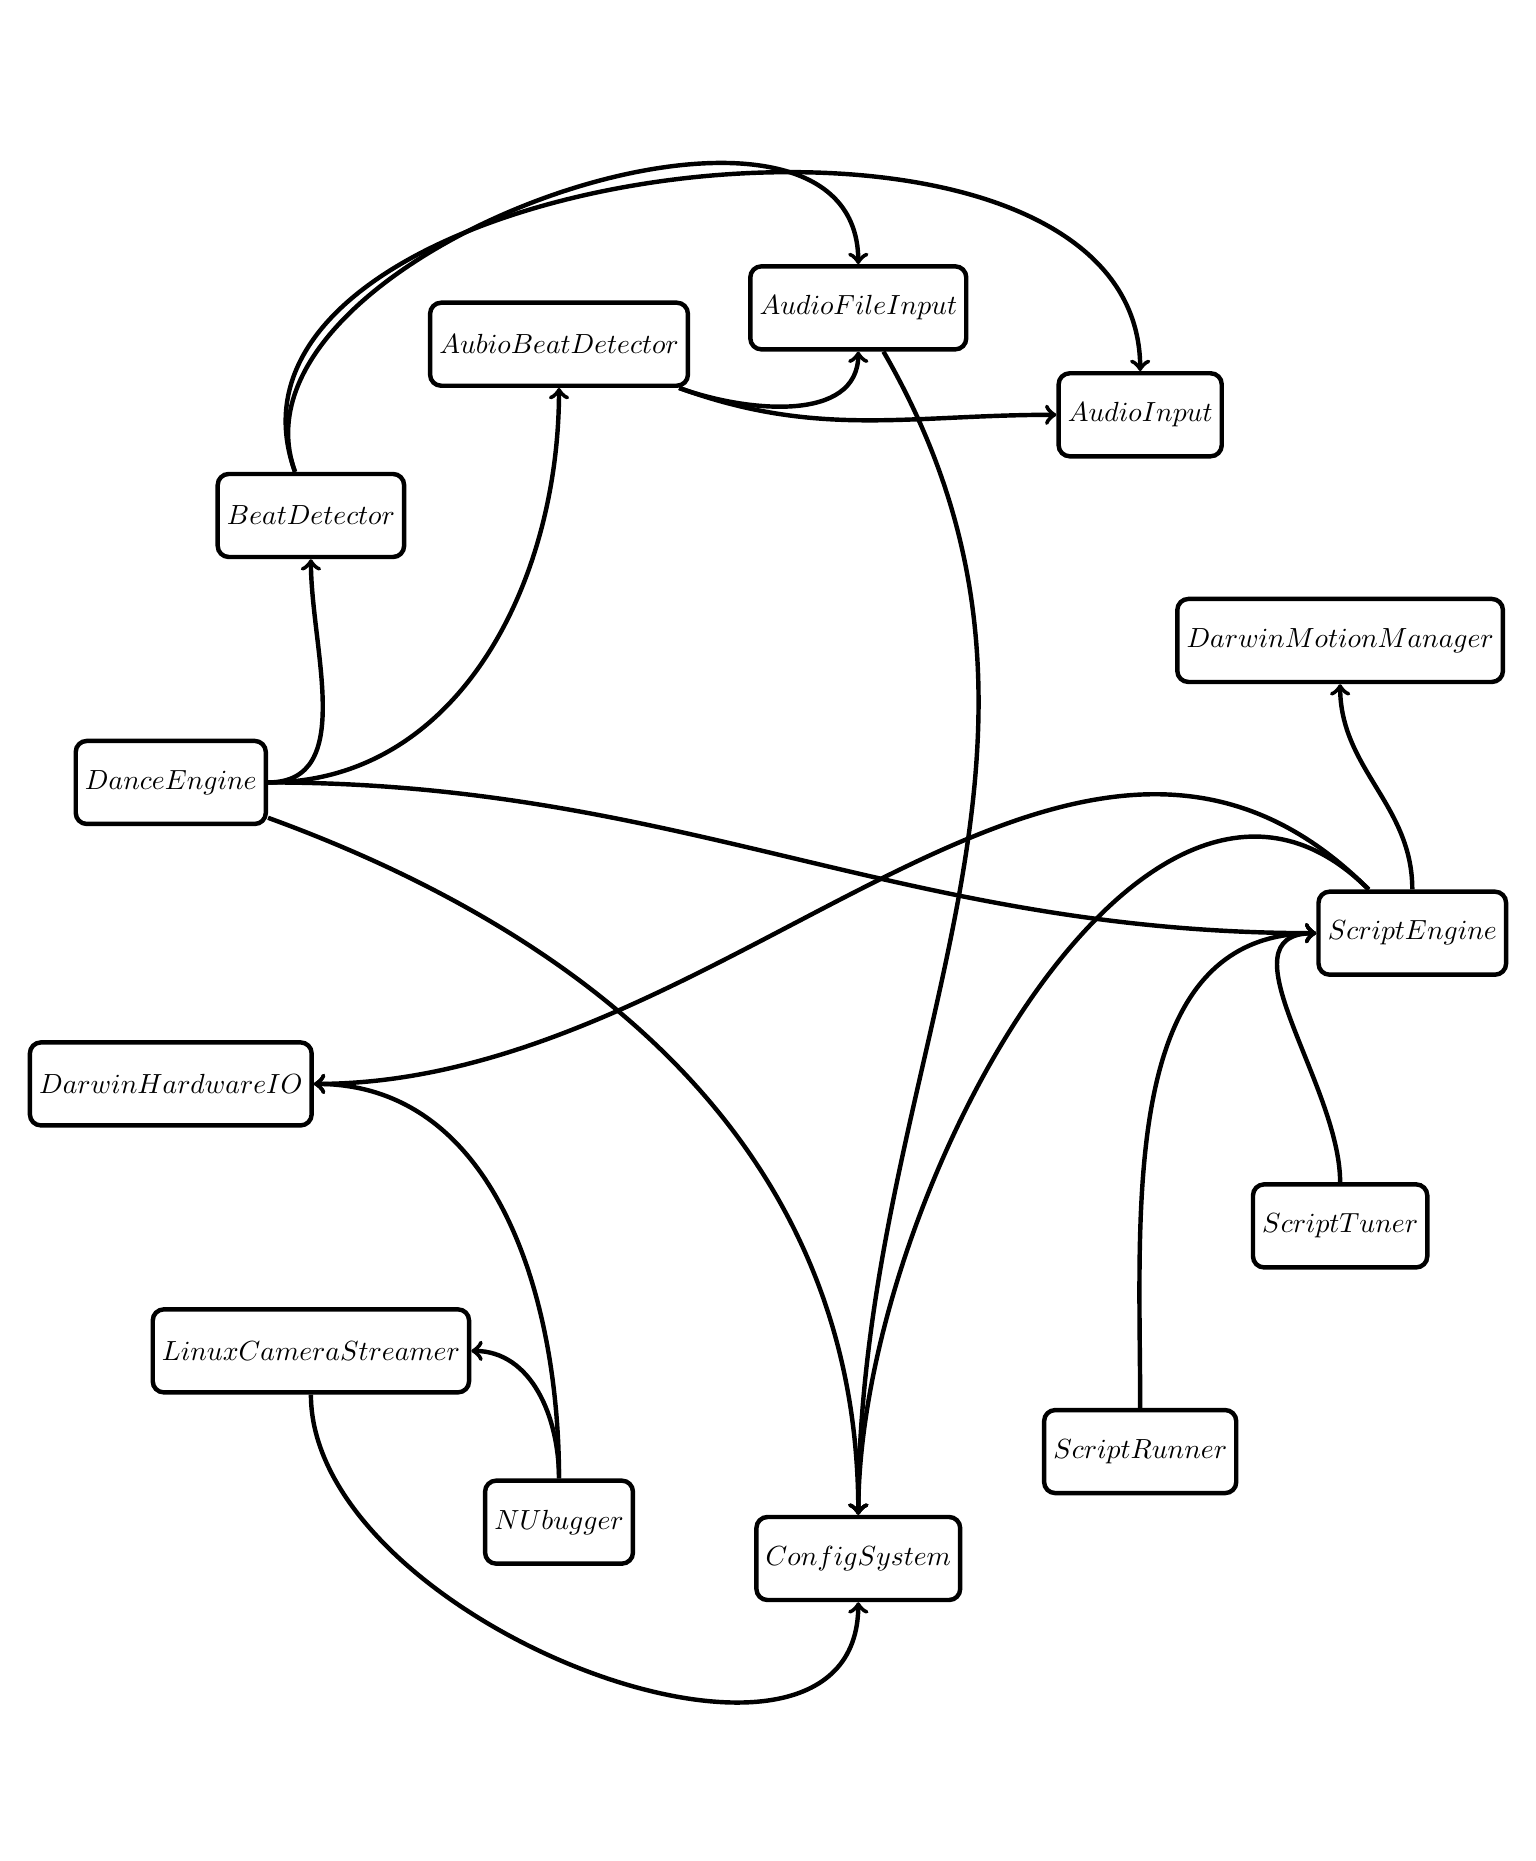
\begin{tikzpicture}[
		reactor/.style={draw, rectangle, rounded corners, minimum height=3em, ultra thick},
		arrow/.style={->, ultra thick}]
		
			%%% Draw all of our components in a circle
			\foreach [count=\i] \reactor in {ScriptEngine,
			                                 DarwinMotionManager,
			                                 AudioInput,
			                                 AudioFileInput,
			                                 AubioBeatDetector,
			                                 BeatDetector,
			                                 DanceEngine,
			                                 DarwinHardwareIO,
			                                 LinuxCameraStreamer,
			                                 NUbugger,
			                                 ConfigSystem,
			                                 ScriptRunner,
			                                 ScriptTuner} {
			
				% Draw the reactors around the central star
				\node[reactor] (\reactor) at ({360/13 * (\i - 1)}:8cm) {$\reactor$};
			};
			
			% Beat detectors use audio inputs
			\path (BeatDetector)        edge[arrow, out=110, in=90] (AudioFileInput) ;
			\path (BeatDetector)        edge[arrow, out=110, in=90] (AudioInput);
			\path (AubioBeatDetector)   edge[arrow, out=340, in=270] (AudioFileInput);
			\path (AubioBeatDetector)   edge[arrow, out=340, in=180] (AudioInput);
			
			% Dance engine uses beat detectors
			\path (DanceEngine)         edge[arrow, out=0, in=270] (BeatDetector);
			\path (DanceEngine)         edge[arrow, out=0, in=270] (AubioBeatDetector);
			
			% Script things use the Script Engine
			\path (ScriptTuner)         edge[arrow, out=90, in=180] (ScriptEngine);
			\path (ScriptRunner)        edge[arrow, out=90, in=180] (ScriptEngine);
			\path (DanceEngine)         edge[arrow, out=0, in=180] (ScriptEngine);
			
			% NUbugger uses the HardwareIO and Camera
			\path (NUbugger)            edge[arrow, out=90, in=0] (LinuxCameraStreamer);
			\path (NUbugger)            edge[arrow, out=90, in=0] (DarwinHardwareIO);
			
			% The Script engine uses motion manager to operate
			\path (ScriptEngine)        edge[arrow, out=90, in=270] (DarwinMotionManager);
			
			% The Motion Manager use HardwareIO
			\path (ScriptEngine)        edge[arrow, out=135, in=0] (DarwinHardwareIO);
			
			% The config system is used by several modules
			\path (AudioFileInput)      edge[arrow, out=300, in=90] (ConfigSystem);
			\path (LinuxCameraStreamer) edge[arrow, out=270, in=270] (ConfigSystem);
			\path (DanceEngine)         edge[arrow, out=340, in=90] (ConfigSystem);
			\path (ScriptEngine)        edge[arrow, out=135, in=90] (ConfigSystem);
			
		\end{tikzpicture}}
		\caption{Integration tests between modules which share arrows can be created as needed}
		\label{fig:links}
	\end{figure}
	
\section{Simulation Testing}
	By implementing modules that simulate the hardware components of the robotic platform, it is possible to perform a full simulation.
	There currently exists two simulation engines that are able to perform high level simulations for the robot system.
	Webots and Simspark are both based on the Open Dynamic Engine (ODE), which is an open source physics and rigid body simulator.
	This allows high level simulations of the robot’s environment. These systems allow testing on the entirety of the robotic system to be performed without requiring physical access to a robot.
	
	Webots or Simspark can be used to provide implementations for the simulated hardware components.
	For the current system, DarwinHardwareIO, DarwinMotionManager, LinuxCameraStreamer and AudioInput can be replaced with simulated equivalents.
	In the case of Webots, the API can be used directly in the modules as Webots provides a C++ API.
	In the case of Simspark, the API is provided using a set of TCP/UDP sockets.
	Instead, modules can be created that read from the sockets and pass the appropriate information to the system.
	Easy integration of the new system into Webots or Simspark provides greater testing capabilities.
\end{document}